% !TEX program = xelatex
\documentclass[11pt,aspectratio=169]{beamer}

\makeatletter
\def\@makefnmark{}
\makeatletter

\setbeamersize{text margin left=5mm,text margin right=5mm} 

\usepackage{amsthm,amsmath,amssymb,braket,fontspec,unicode-math}
\usepackage[absolute,overlay]{textpos}

\usetheme[numbering=none,nofirafonts]{focus}

\setbeamercolor{footnote}{fg=blue}
\setbeamerfont{footnote}{size=\tiny}

\setmainfont{FiraCode Nerd Font}
\setsansfont{Fira Sans}
\setmathfont{Fira Math}
\setmathfont{Latin Modern Math}[range={frak,\bigcap,\bigcup}]
\setbeamerfont{title}{size=\LARGE, shape=\scshape}
\setbeamerfont{author}{size=\large, shape=\scshape}
\setbeamerfont{institute}{size=\normalsize, shape=\scshape}
\setbeamerfont{date}{size=\normalsize, shape=\scshape}
\setbeamerfont{frametitle}{size=\large, shape=\scshape}

\usepackage[backend=bibtex,url=false,doi=false,maxcitenames=1, style=authoryear]{biblatex}
\bibliography{bib}
\AtBeginBibliography{\scriptsize}

\newcommand{\focus}[1]{\textcolor{red}{\bf{#1}}}

\definecolor{red}{HTML}{CC0000}
\definecolor{lred}{HTML}{e24a33}
\definecolor{lblue}{HTML}{348abd}
\setbeamertemplate{bibliography item}[triangle]

\graphicspath{{./figures/}} % Change the path

\AtBeginSection[]{
  \vfill
  \centering
  \begin{beamercolorbox}[sep=20pt,rounded=true,center]{frametitle}
    \usebeamerfont{title}\insertsectionhead\par%
  \end{beamercolorbox}
  \vfill
}
\title{Emergence in free and correlated fermions: from impurity models to the bulk}

\subtitle{RPC Presentation 2021-22}

\date{\today}
\author{Abhirup Mukherjee\\Supervisor: Dr. Siddhartha Lal}
\institute{Department of Physical Sciences, IISER Kolkata, Mohanpur}
\date{\today}
     
\begin{document}

\centering

\begin{frame}
\maketitle
\begin{textblock*}{0.4\textwidth}(5.5cm, 6.5cm)
	\centering
	\vspace*{\fill}

	
\includegraphics[width=0.35\textwidth]{figures/epqm_logo_mod.jpeg}
	\hspace*{\fill}
	
\includegraphics[width=0.35\textwidth]{figures/dps_logo.jpeg}

	\vspace*{\fill}
\end{textblock*}
\end{frame}

\begin{frame}{}
\section{Summary of Work}
\end{frame}

\begin{frame}{Summary of Work}
\begin{enumerate}
\item 1-channel Kondo problem: {\it as second author}, {published} in Phys. Rev. B\\
	\focus{Phys. Rev. B 105, 085119}\\[20pt]
	\item Multi-channel Kondo problem: {\it as second author}, {under review} at Phys. Rev. B\\
		\focus{arXiv:2205.00790}\\[20pt]
	\item Generalised Anderson impurity model: manuscript \focus{in preparation}\\[20pt]
	\item Entanglement scaling in free fermions: manuscript \focus{in preparation}\\[20pt]
	\item New auxiliary model approach to correlated systems: \focus{ongoing project}
\end{enumerate}

\end{frame}

\begin{frame}{}
\section{Single-channel Kondo problem}
\small{Phys. Rev. B 105, 085119\\[10pt]
Anirban Mukherjee, {\bf Abhirup Mukherjee}, N. S. Vidhyadhiraja, A. Taraphder, and Siddhartha Lal}
\end{frame}

\begin{frame}{Single-channel Kondo problem}
\footcite{kondo1964resistance,wilson1975,andreiKondoreview,hewson1993,nozieres1974fermi,anderson1970,tsvelickKondoreview,affleck1993exact,Goldhaber-Gordon1998,Borzenets2020,sakai_osamu_shimizu,costi_hewson_1990,nozaki2012,affleck1995conformal}
Model of impurity interacting with conduction electrons through spin-flips\\[20pt]

\begin{minipage}{0.59\textwidth}
\begin{enumerate}
\item Computation of the impurity spectral function\\[20pt]
\item Emergence of a local Fermi liquid, and orthogonality catastrophe between local moment and singlet states\\[20pt]
\item Calculating of thermal entropy\\[20pt]
\end{enumerate}
\end{minipage}
\begin{minipage}{0.4\textwidth}
	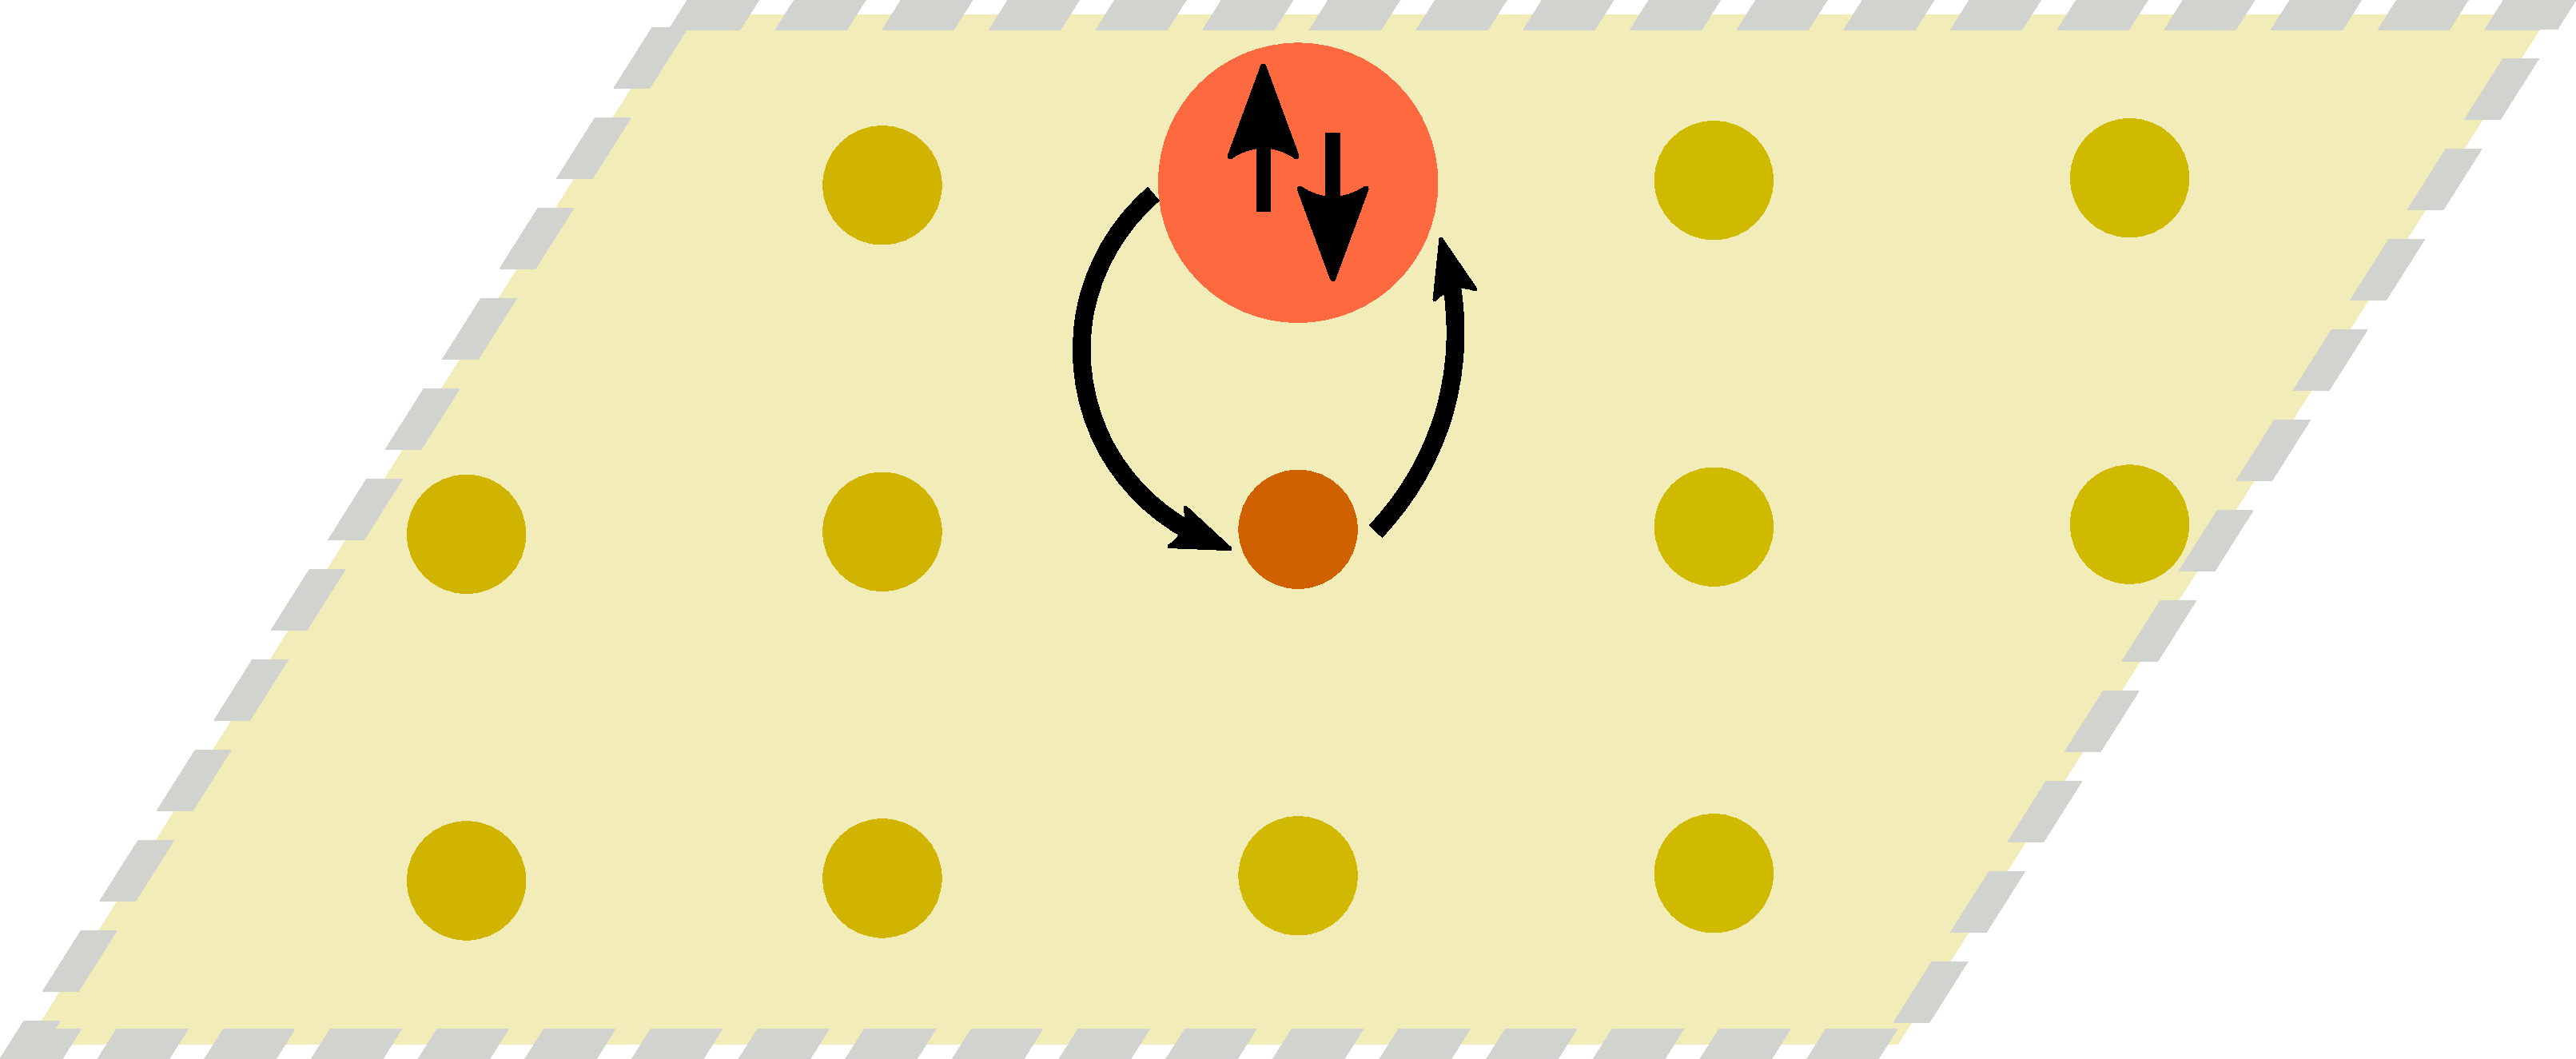
\includegraphics[width=\textwidth]{kondo-effect.pdf}
\end{minipage}

\end{frame}

\begin{frame}{}
\section{Multi-channel Kondo problem}
\small{arXiv:2205.00790\\[10pt]
Siddhartha Patra, {\bf Abhirup Mukherjee}, Anirban Mukherjee, N. S. Vidhyadhiraja, A. Taraphder, Siddhartha Lal}
\end{frame}

\begin{frame}{Multi-channel Kondo problem}
\footcite{Noz_blandin_1980,Tsvelick_weigmann_mchannel_1985,affleck1993exact,Gan_mchannel_1994,affleck_1991_overscreen,emery_kivelson,bulla_1998}
Model of impurity interacting with multiple conduction electron channels \\[20pt]

\begin{minipage}{0.59\textwidth}
	\begin{enumerate}
		\item Obtaining RG fixed point Hamiltonian\\[20pt]
	\item Analytical forms for degree of compensation, magnetization and susceptibility\\[20pt]
	\item Presence of a local marginal Fermi liquid\\[20pt]
	\item Dualities of the MCK model
\end{enumerate}
\end{minipage}
\begin{minipage}{0.4\textwidth}
	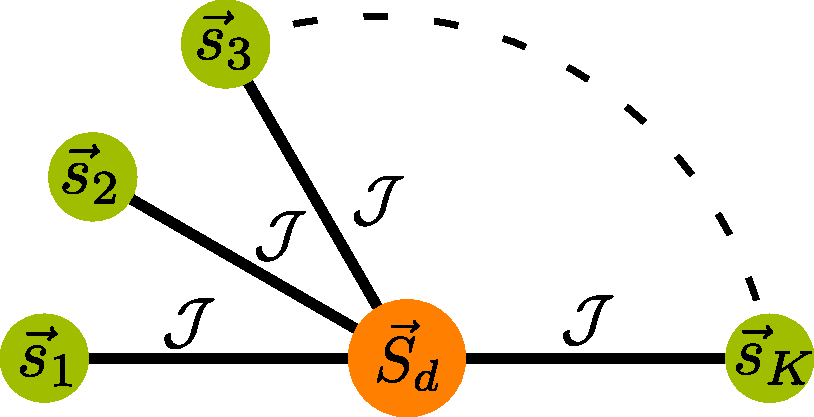
\includegraphics[width=\textwidth]{stargraph.pdf}
\end{minipage}

\end{frame}

\begin{frame}{}
\section{Local metal-insulator transition in extended Anderson impurity model}
\end{frame}

\begin{frame}{Extended Anderson impurity model}
\footcite{anderson_1961,hrk_wilson_1980,hewson1993}
Standard Anderson impurity model \(\longrightarrow\) only one stable phase (strong-coupling) \\[10pt]
\focus{no possibility of phase transition} \(\longrightarrow\) Introduce additional correlation\\[20pt]
\begin{itemize}
	\item spin-flip correlation between impurity and bath: \(J\)
	\item local correlation in the bath: \(U_b\)
\end{itemize}

\vspace*{\fill}

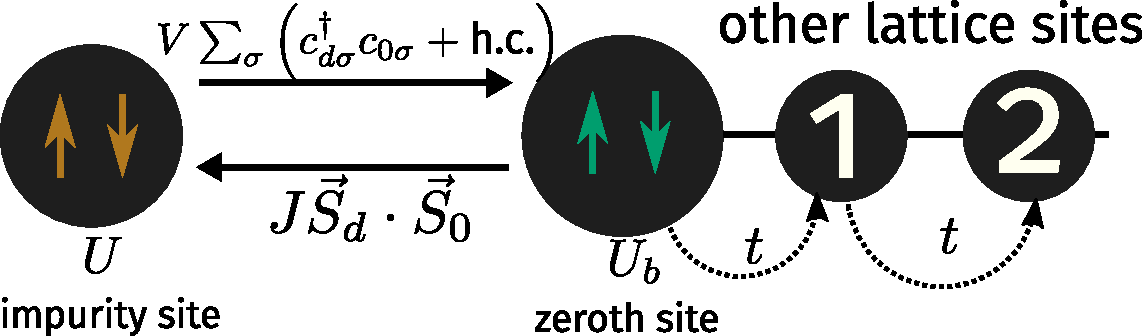
\includegraphics[width=0.6\textwidth]{zeromode_bare.pdf}

\end{frame}

\begin{frame}{RG Phase Diagram}
RG equations reveal critical point where \(J,V\) \focus{become irrelevant}\\[10pt]

\hspace*{-20pt}
\begin{minipage}{0.52\textwidth}
\begin{enumerate}
	\item orange phase: \(J\) is relevant: strong-coupling\\[20pt]
	\item blue phase: \(J\) is irrelevant: local moment\\[20pt]
	\item yellow phase: spin+charge liquid\\[20pt]
	\item gray phase: all couplings irrelevant
\end{enumerate}
\end{minipage}
\begin{minipage}{0.5\textwidth}
	\[r = -U_b/J\]
	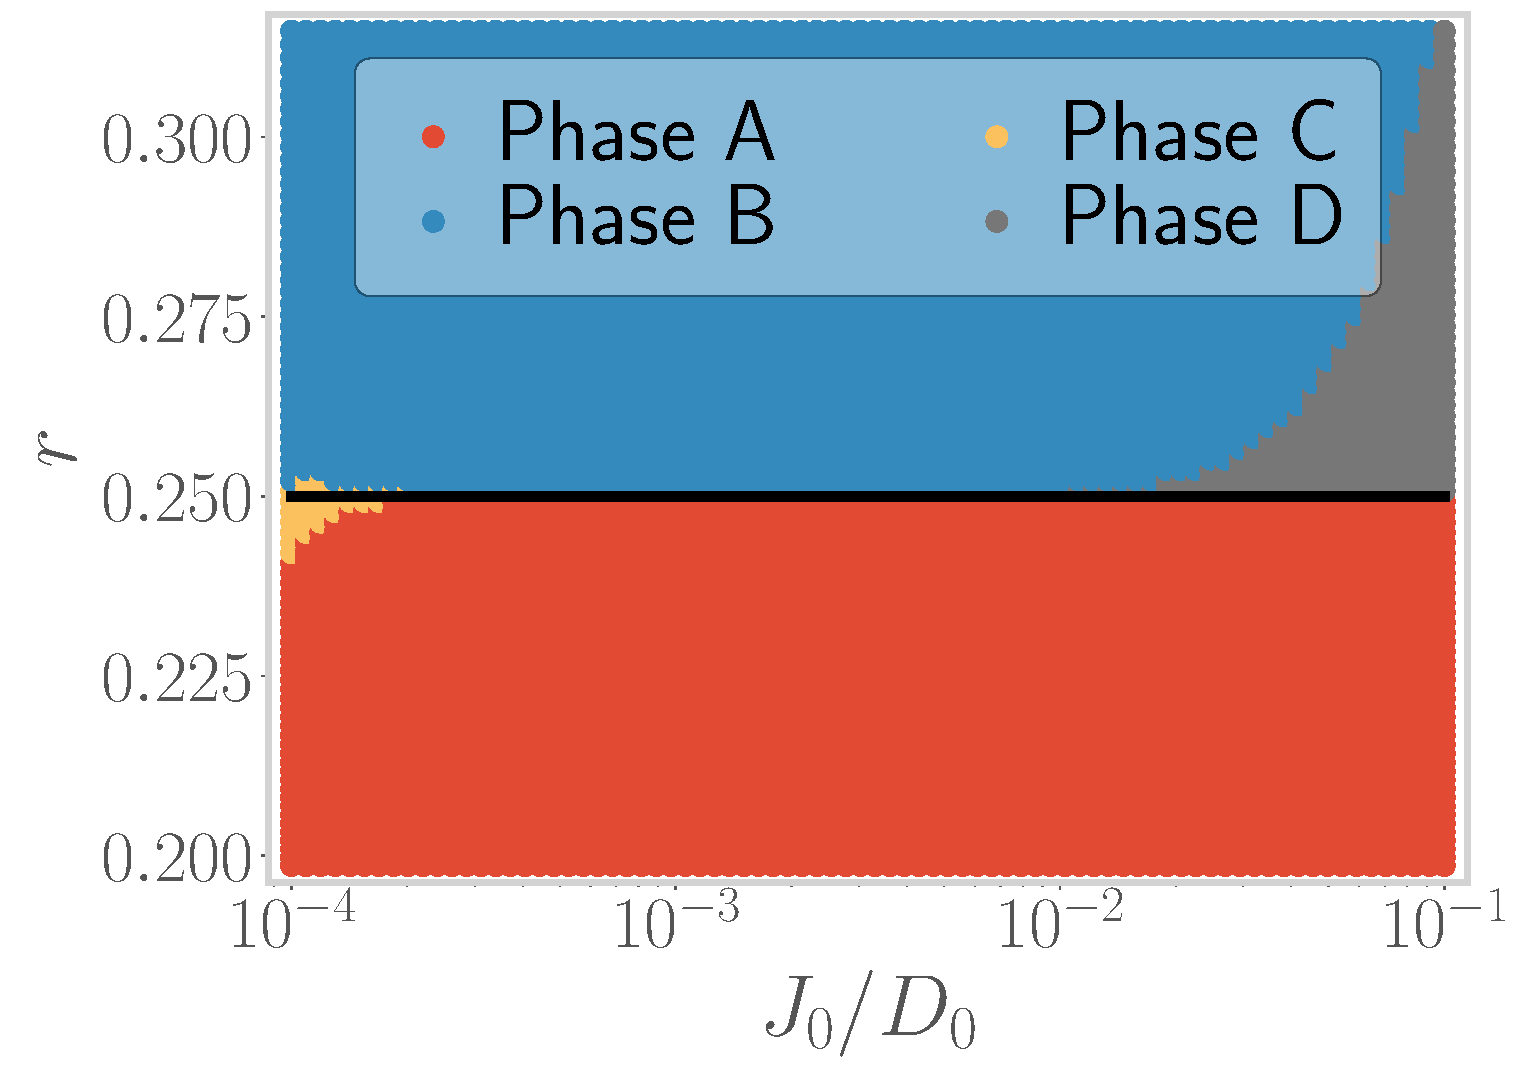
\includegraphics[width=\textwidth]{phase-map-MIT.pdf}
\end{minipage}

\end{frame}

\begin{frame}{Presence of a phase transition}

\begin{minipage}{0.7\textwidth}
singlet {\LARGE \(\longrightarrow\)} spin+charge liquid {\LARGE \(\longrightarrow\)} local moment\\[10pt]
impurity spectral function gaps out
\end{minipage}
\begin{minipage}{0.29\textwidth}
\[r = -U_b/J\]
\[\ket{SS} = \ket{\uparrow,\downarrow} - \ket{\downarrow,\uparrow}\]
\[\ket{CT} = \ket{2,0} + \ket{0,2}\]
\end{minipage}

\vspace*{\fill}

\begin{minipage}{0.49\textwidth}
	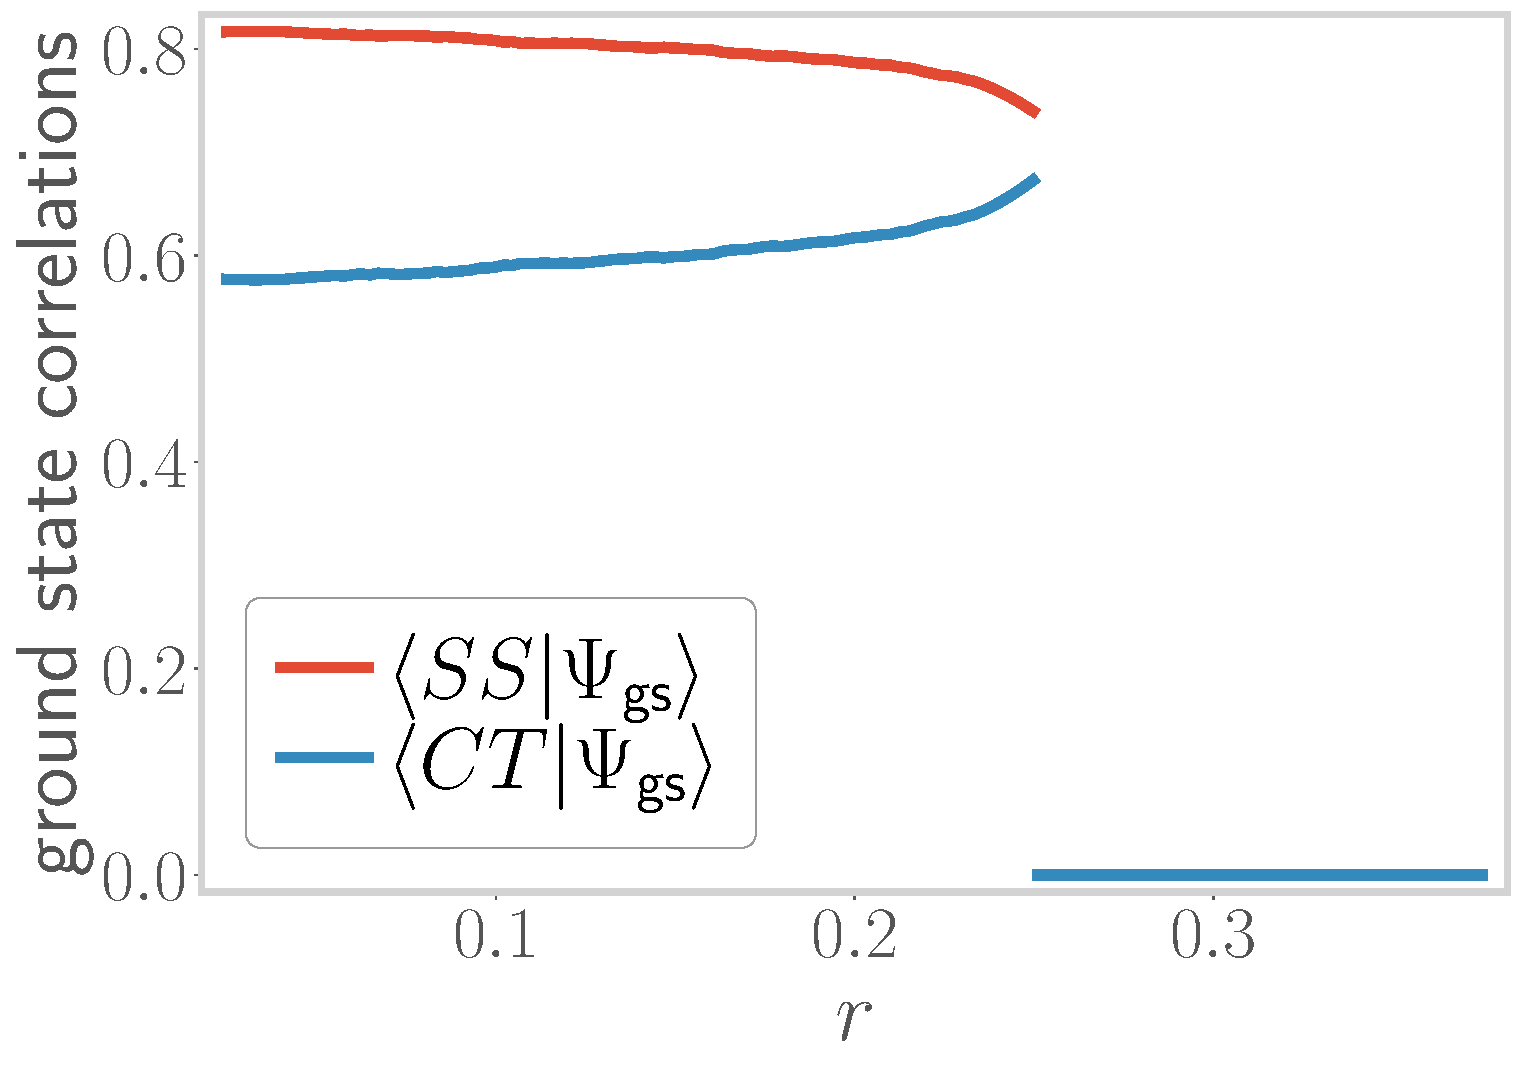
\includegraphics[width=\textwidth]{corrs_gs.pdf}
\end{minipage}
\hspace*{\fill}
\begin{minipage}{0.49\textwidth}
	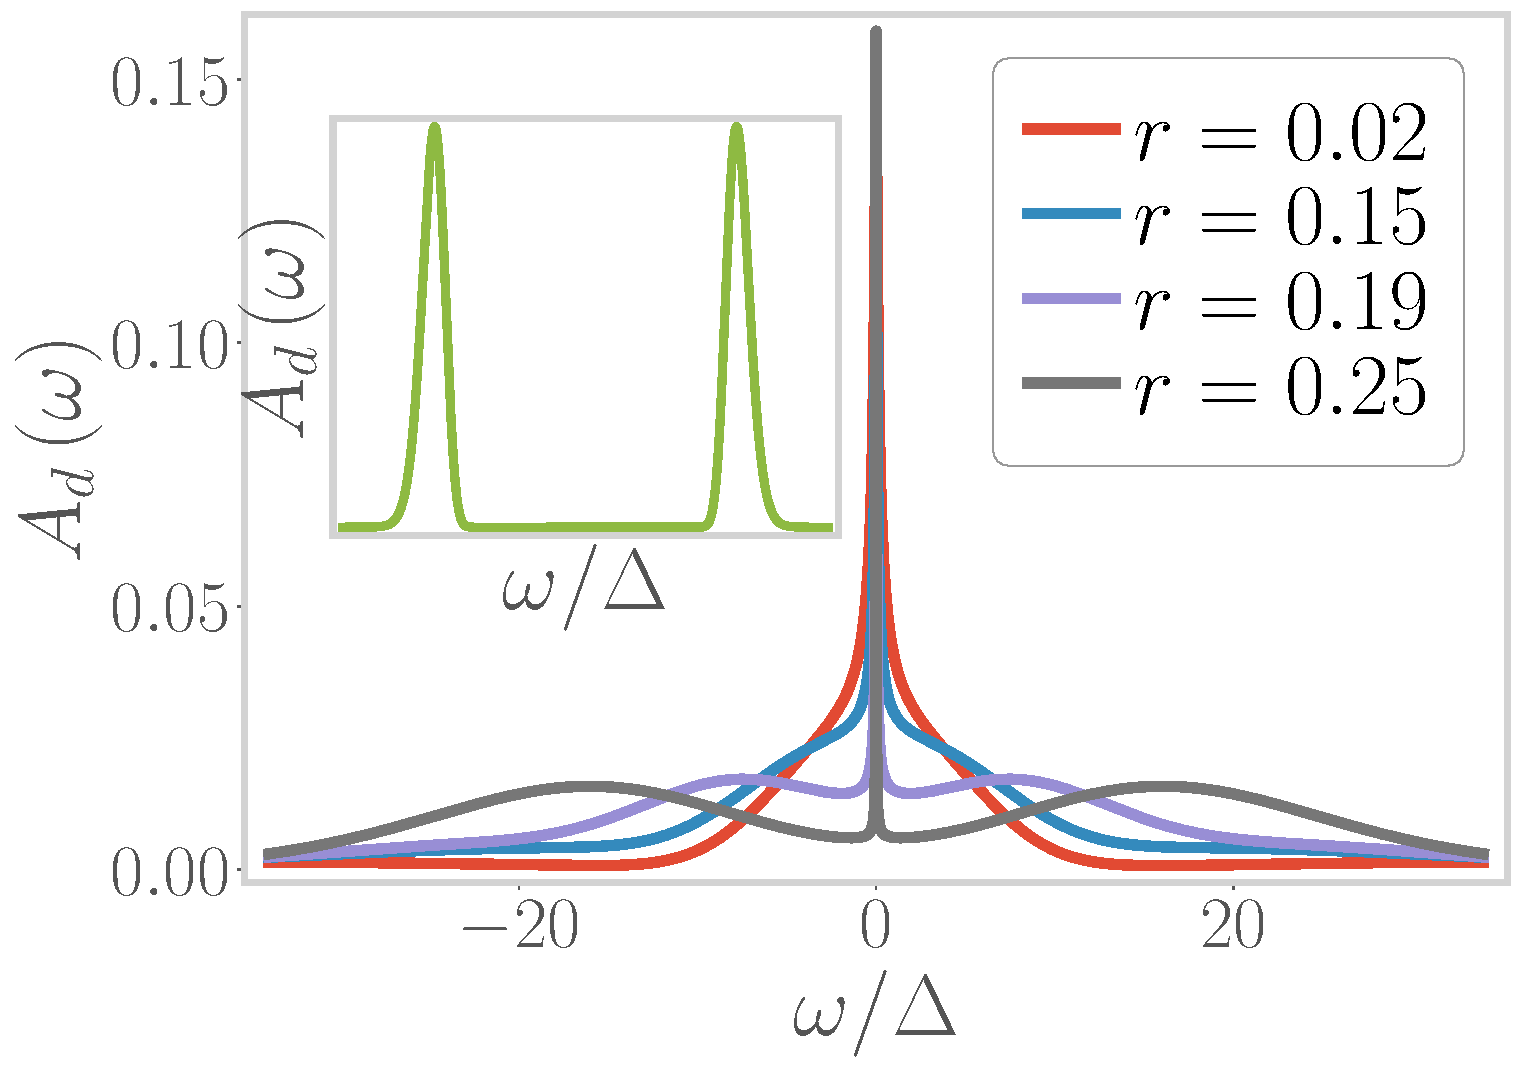
\includegraphics[width=\textwidth]{Add.pdf}
\end{minipage}

\end{frame}

\begin{frame}{Entanglement as a probe for the transition}

	Geometric entanglement: ~ \(\varepsilon(\psi_1,\psi_2) = 1 - |\braket{\psi_1|\psi_2}|^2\)\\[10pt]
	\(\longrightarrow \sqrt{1 -\varepsilon_\text{SS}}\sqrt{1 -\varepsilon_\text{CT}}\) is maximised, then vanishes\\[10pt]
	Mutual information between impurity and cloud vanishes\\[10pt]

\begin{minipage}{0.49\textwidth}
	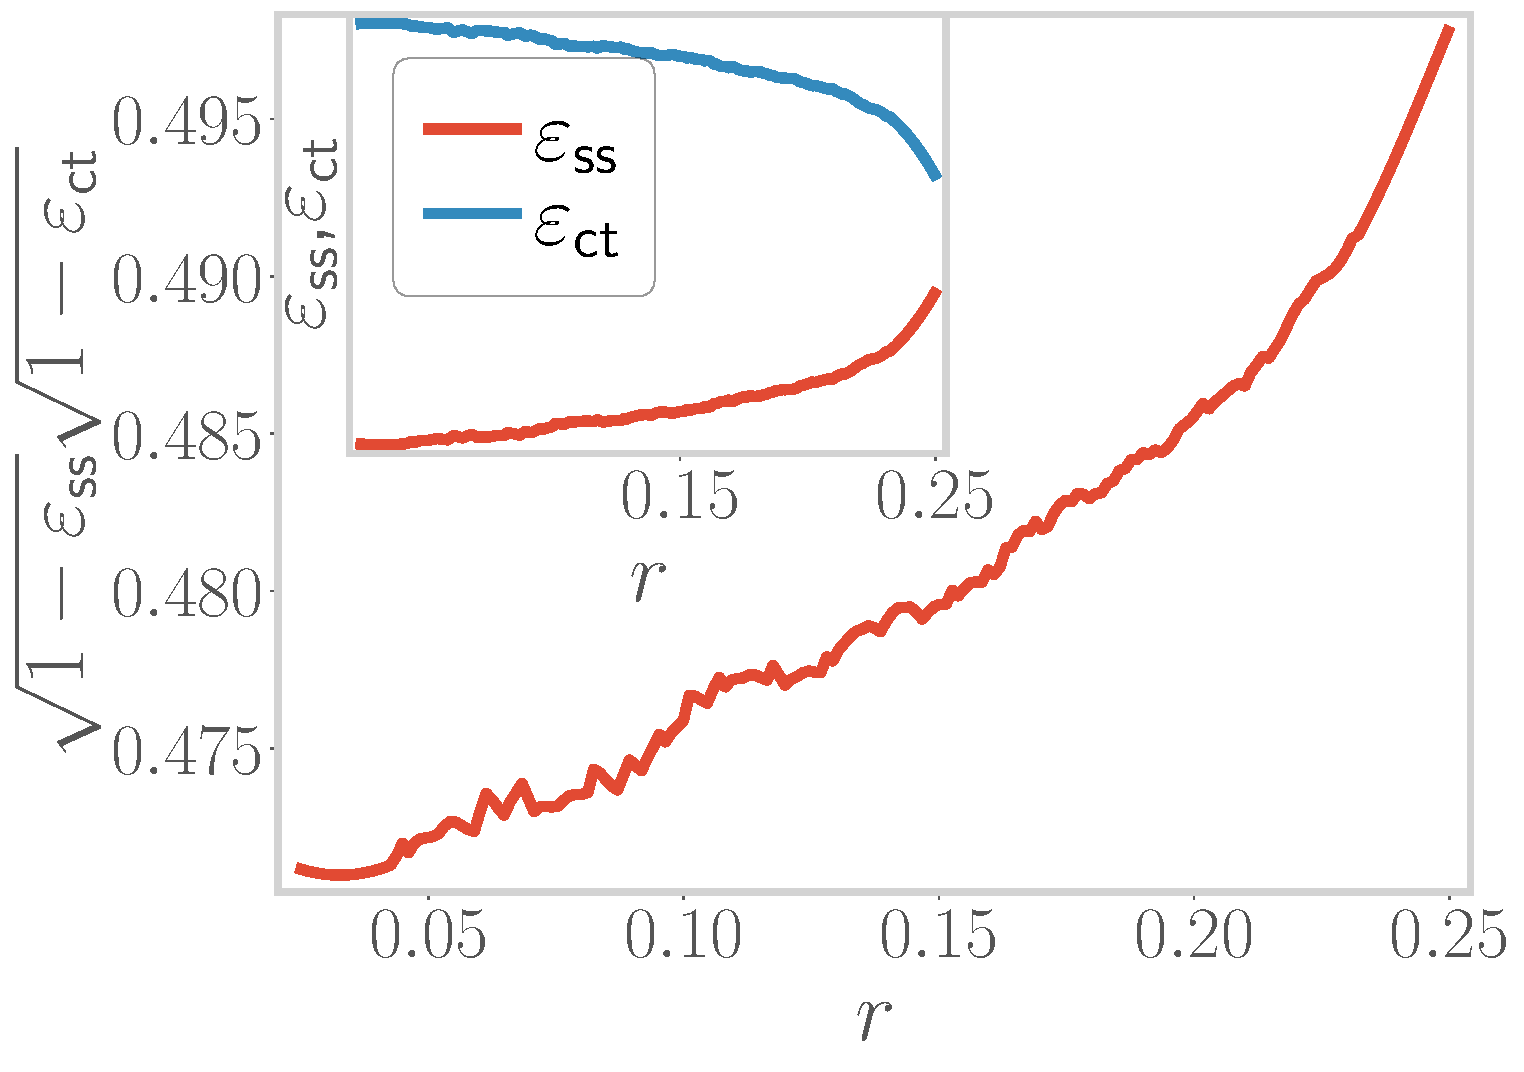
\includegraphics[width=\textwidth]{entanglement.pdf}
\end{minipage}
\hspace*{\fill}
\begin{minipage}{0.49\textwidth}
	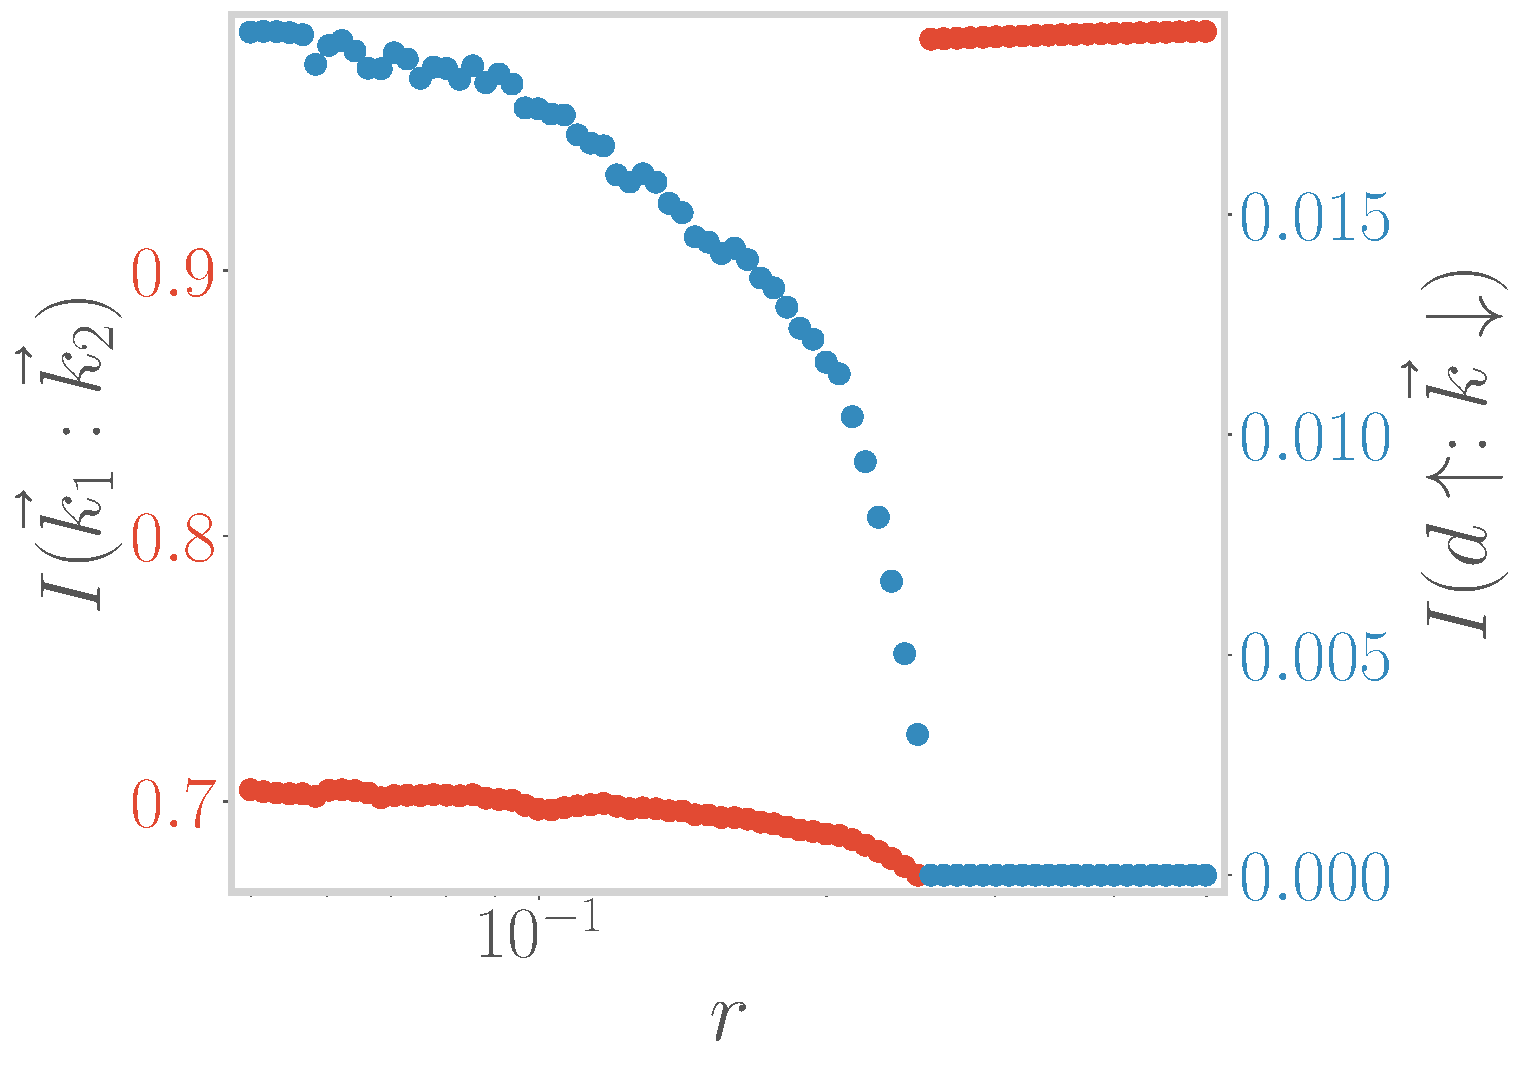
\includegraphics[width=\textwidth]{I_k.pdf}
\end{minipage}

\end{frame}

\begin{frame}{Presence of subdominant pair fluctuations}
	
\begin{itemize}
	\item \focus{pairing tendencies} observed near the quantum critical point\\[10pt]
	\item might lead to \focus{superconductivity} with doping\\[10pt]
	\item seen in cuprates, heavy-fermions materials, pnictides, etc\\[10pt]
\end{itemize}
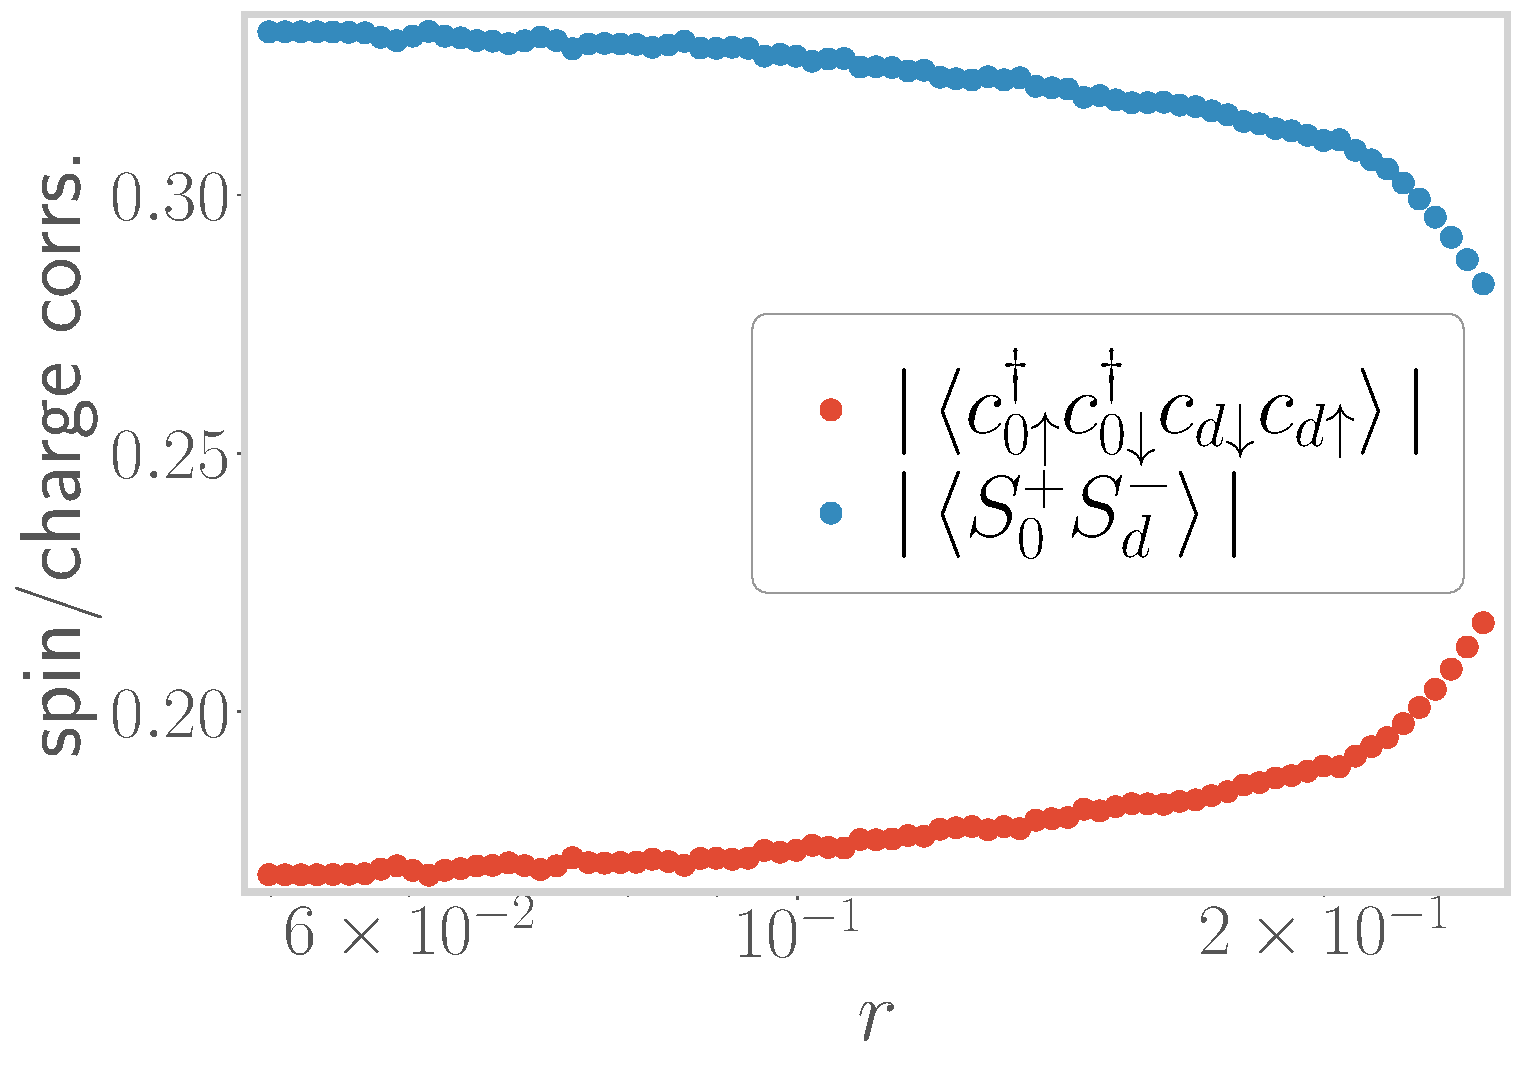
\includegraphics[width=0.45\textwidth]{odlro_d0.pdf}
\hspace*{\fill}
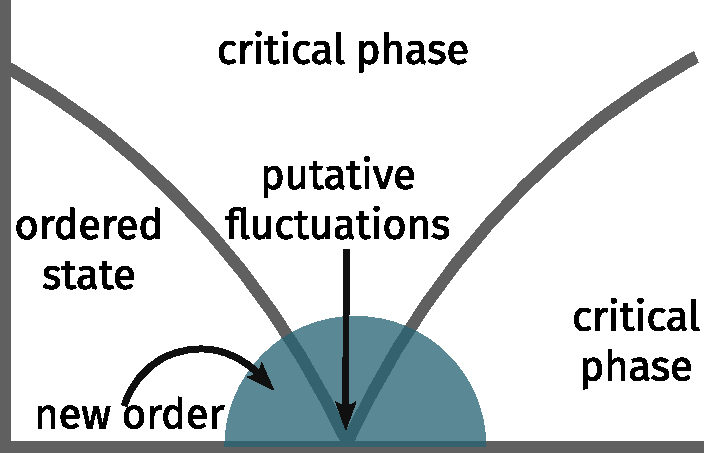
\includegraphics[width=0.45\textwidth]{gen-phase-diagram.pdf}
\end{frame}



\begin{frame}{}
\section{Entanglement scaling in free fermions}
\end{frame}

\begin{frame}{Creating subsystems}
	\[\text{Free Dirac fermions on torus:}~ ~ ~ k_x^n = \frac{2\pi }{L_x} n,~ ~ n \in \mathbb{Z};~~~ \text{define \focus{sparsity}} = \Delta n = 1\]
	\focus{Simplest} choice: the entire set
	\[\text{sparsity} = 1 \longrightarrow n \in \left\{-N,-(N-1),-(N-2),\ldots,-1,0,1,\ldots,N-2,N-1,N\right\} \]
	\focus{Coarser} choices: increase sparsity
	\[\text{sparsity} = 2 \longrightarrow n \in \left\{-N,-(N-2),-(N-4),\ldots,-2,0,2,\ldots,N-4,N-2,N\right\} \]
	\[\text{sparsity} = 4 \longrightarrow n \in \left\{-N,-(N-4),-(N-8),\ldots,-4,0,4,\ldots,N-8,N-4,N\right\} \]
	\centering
	\vspace*{\fill}
	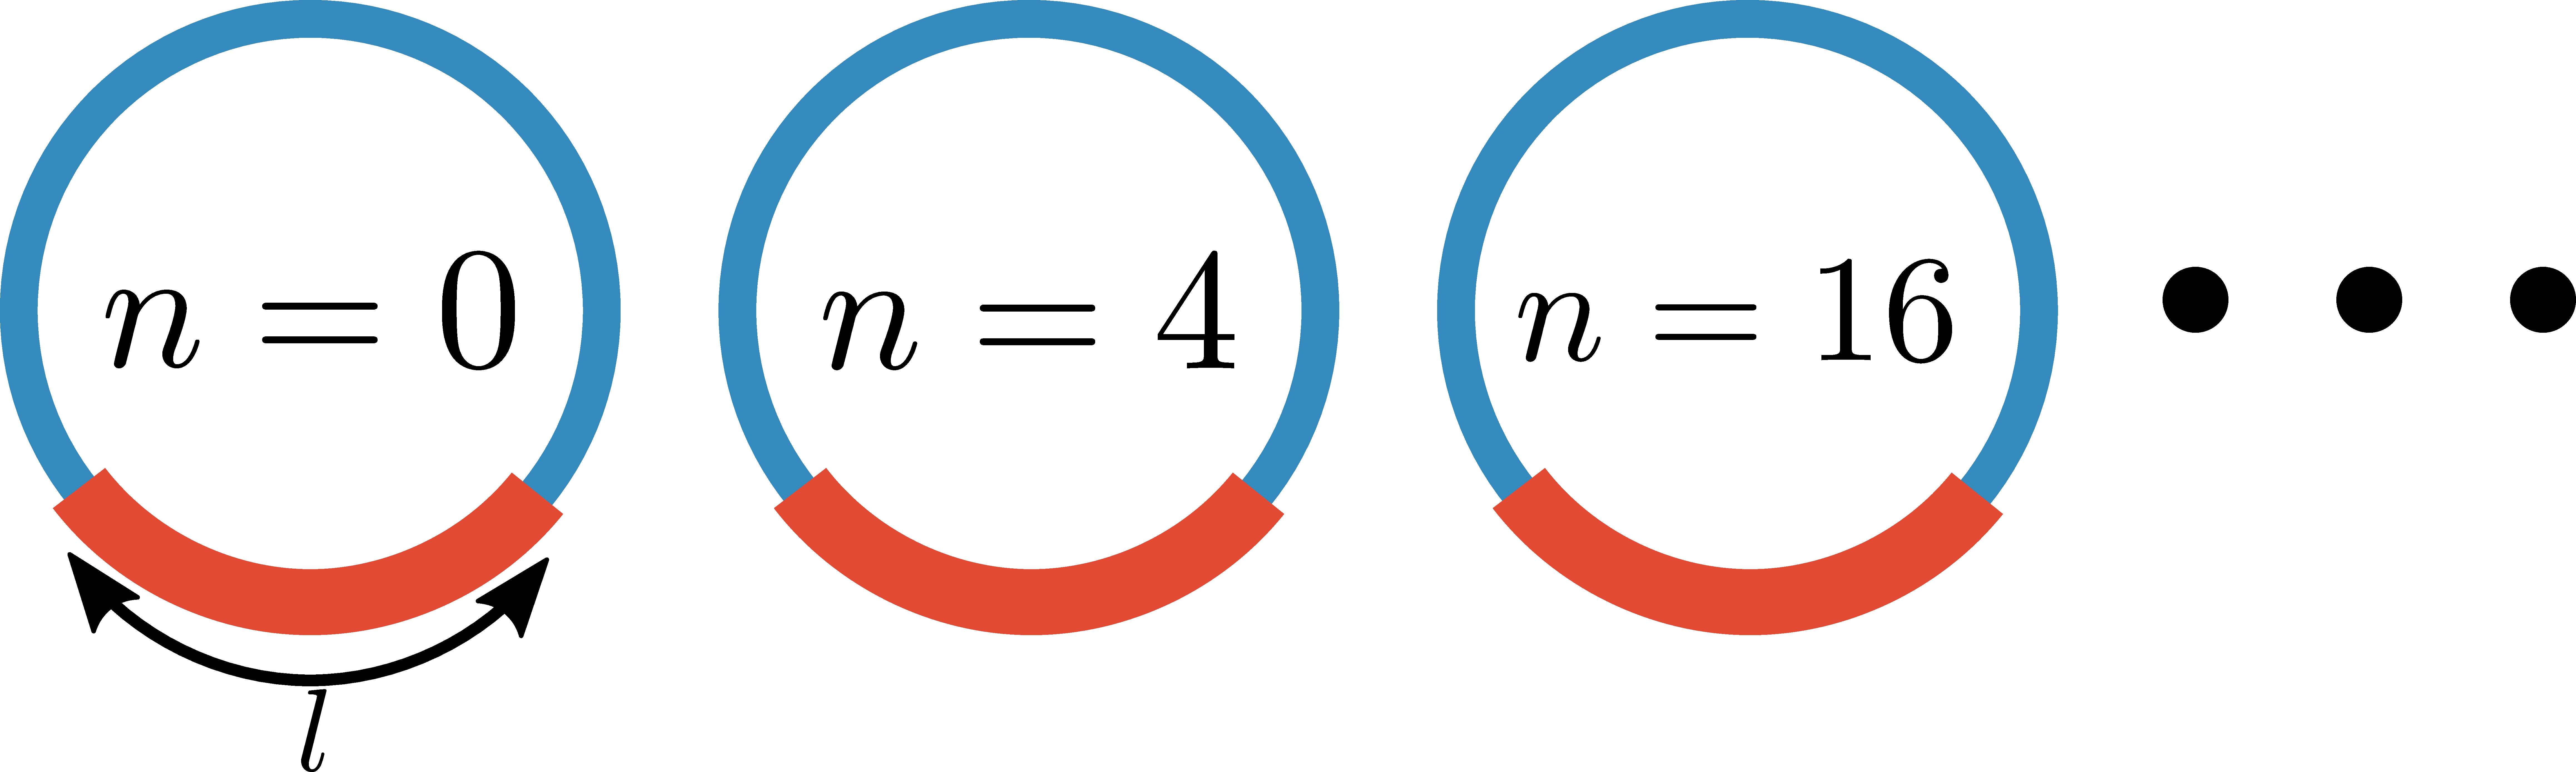
\includegraphics[width=0.4\textwidth]{figures/A_mi.pdf}
	\hspace*{\fill}
	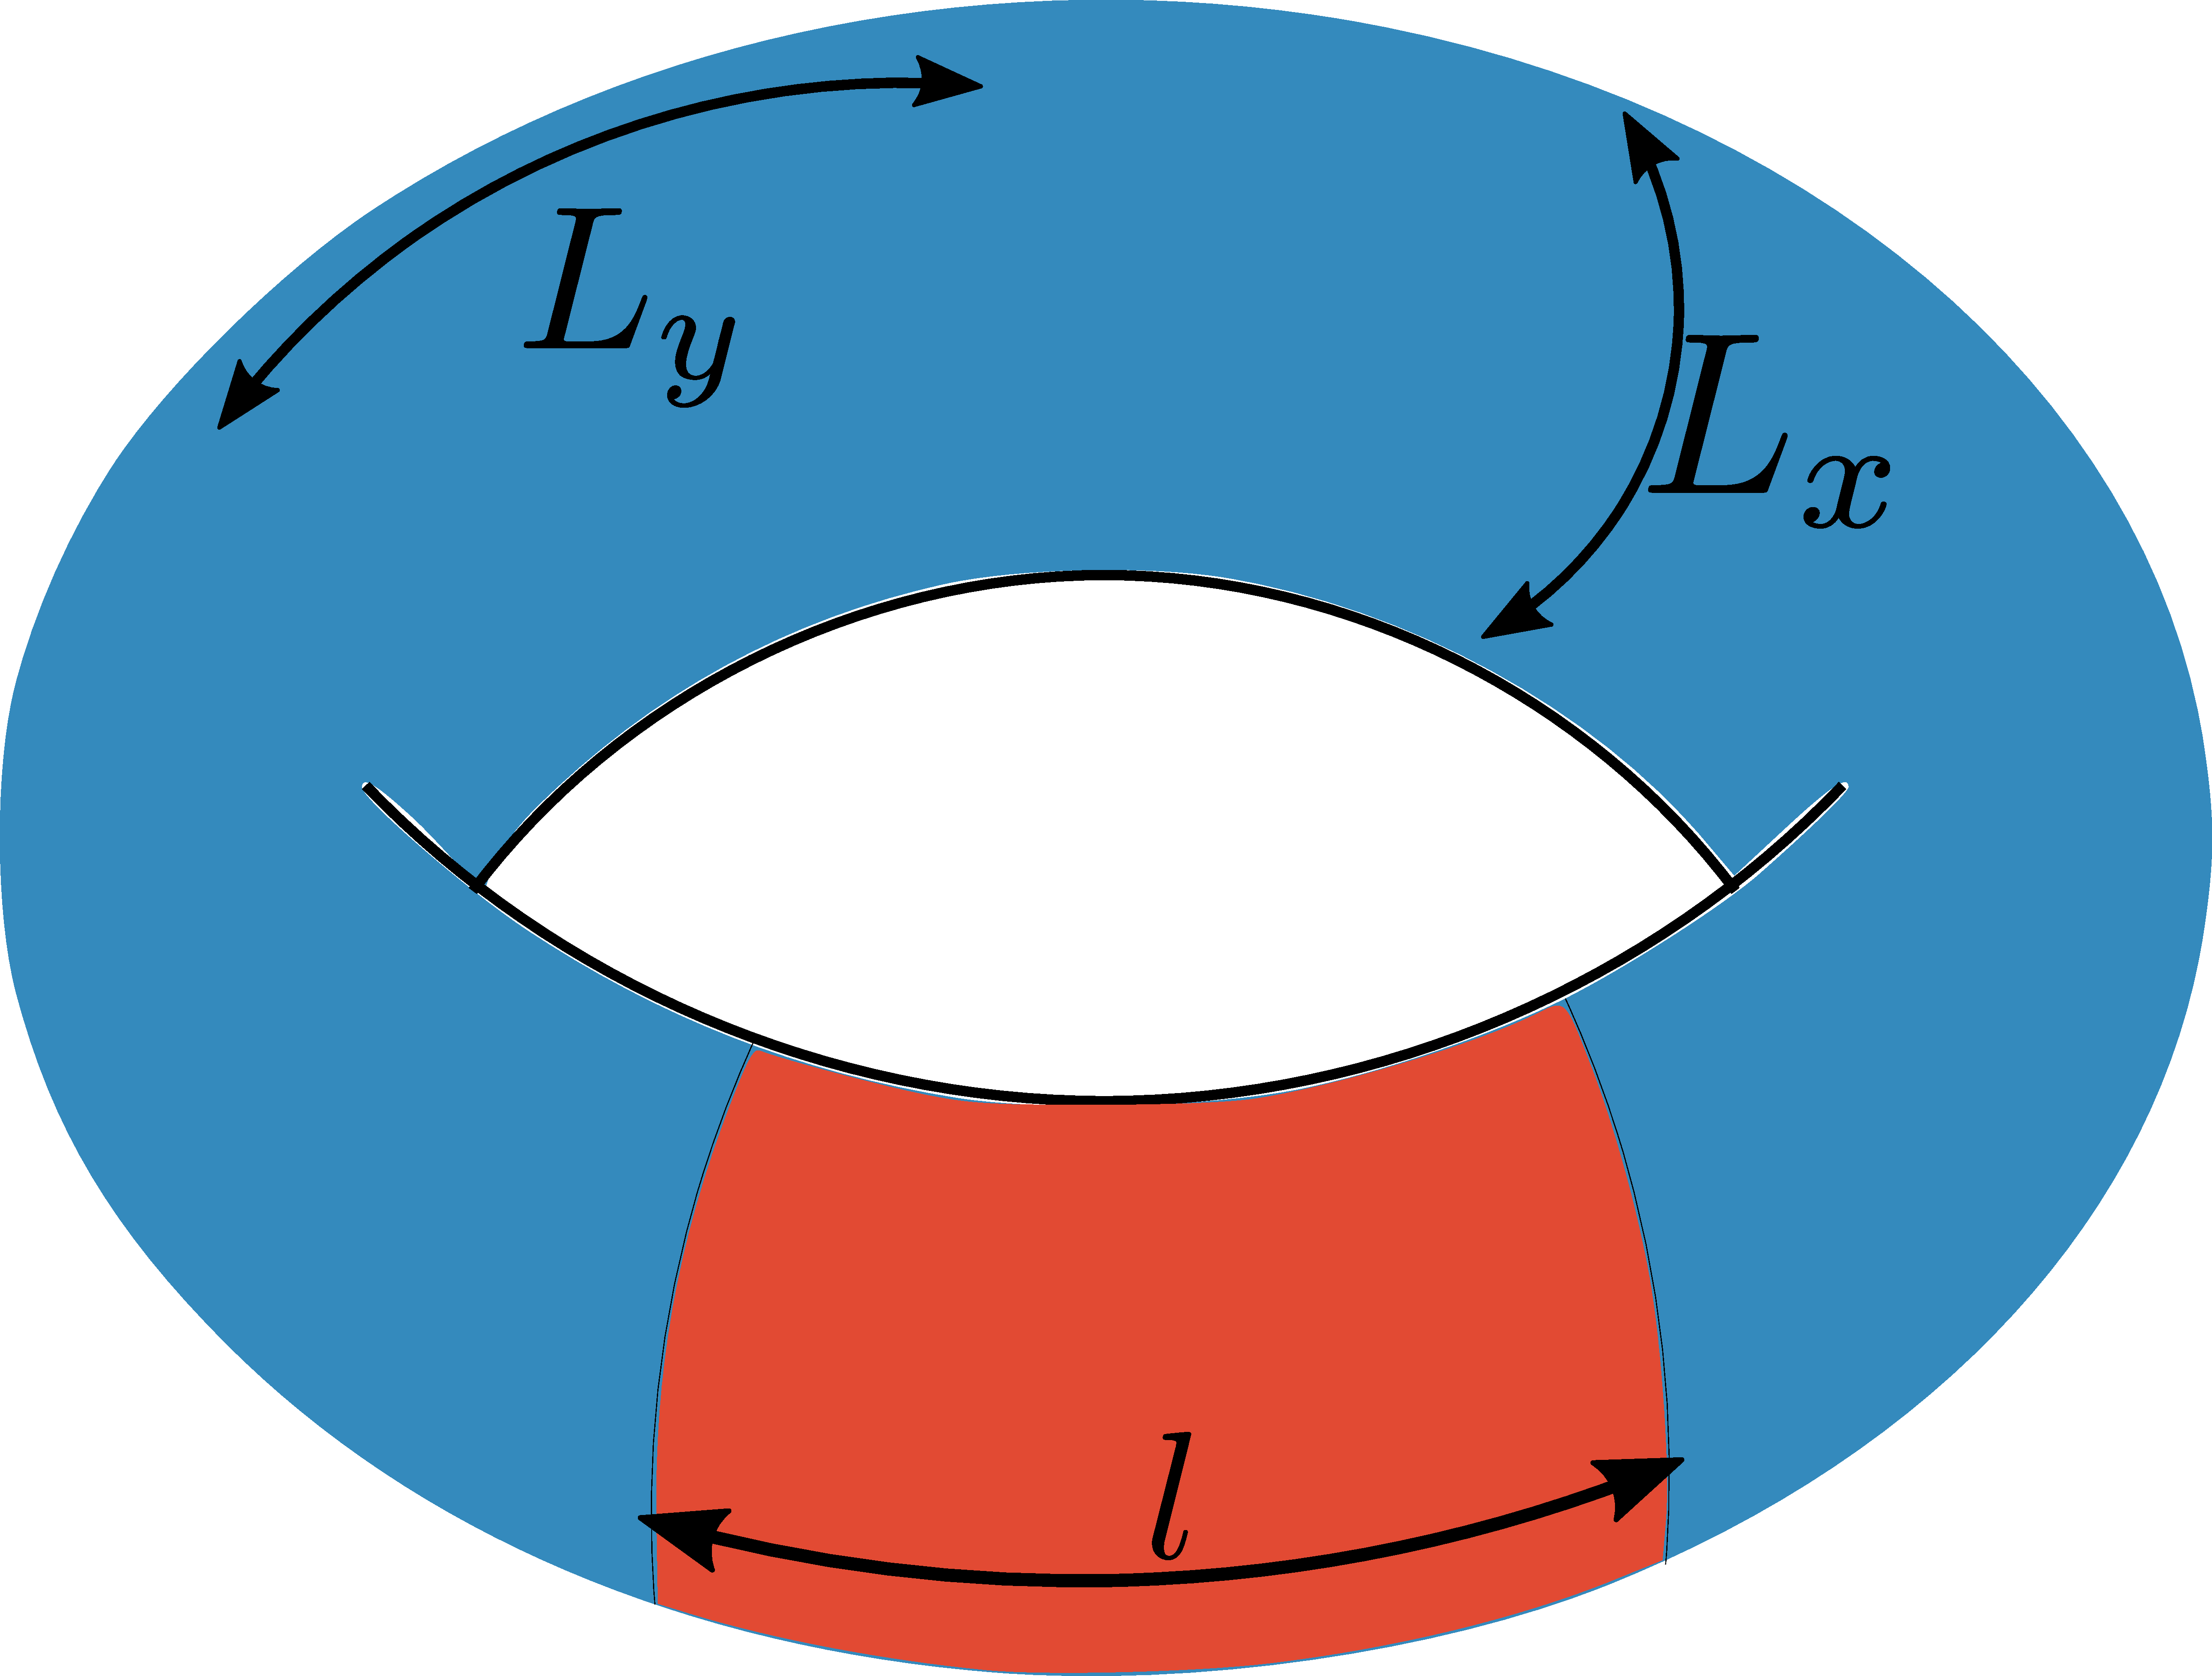
\includegraphics[width=0.25\textwidth]{figures/subsystem-torus.pdf}
\end{frame}

\begin{frame}{Subsystem entanglement entropy: Entanglement hierarchy}
\footcite{Calabrese_2004,Casini_2005,Arias_2015,Chen_2017,Murciano_2020}
\begin{minipage}{0.5\textwidth}
\[S_{\mathcal{A}_z(j)} = f_z(j) c \alpha L_x - c \log \big|2\sin\left(\pi f_z(j)\phi\right)\big|\]
\[i < j, ~ ~ S_{i\cup j} =
	\begin{cases}
	S_{i}, ~ ~ z > 0\\
	S_{j}, ~ ~ z < 0
	\end{cases}
\]
\end{minipage}
\begin{minipage}{0.45\textwidth}
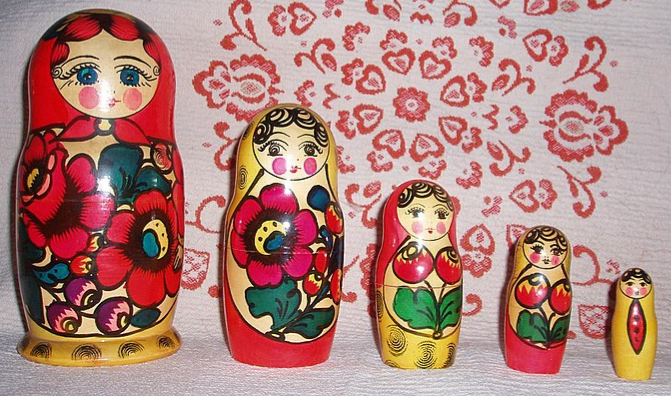
\includegraphics[height=0.3\textheight]{figures/Matroshka.png}
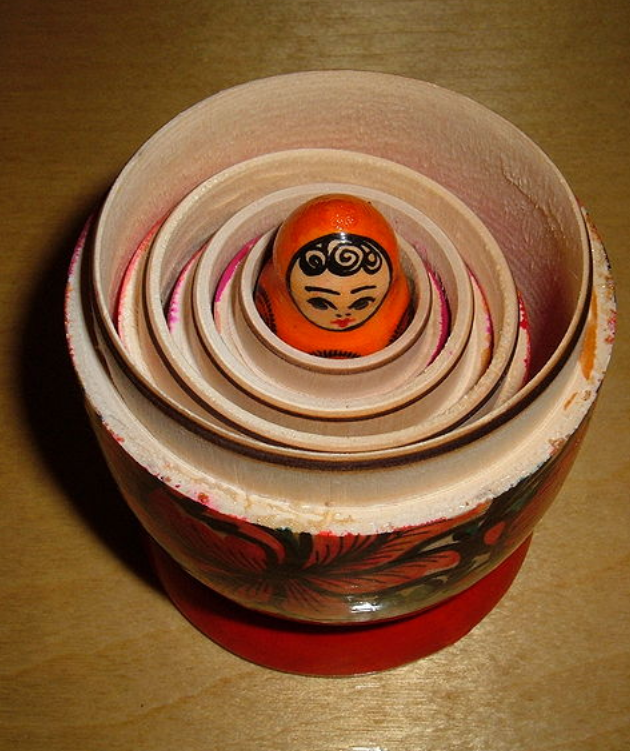
\includegraphics[height=0.3\textheight]{figures/nested.png}
\end{minipage}

\vspace*{\fill}

\begin{itemize}
	\item 
presents a \focus{hierarchy} of entanglement \(\longrightarrow\) EE distributed across RG steps\\
RG transformation \(\longrightarrow\) reveals entanglement

\vspace*{\fill}
\item distribution of entanglement also present in \focus{multipartite} entanglement
\end{itemize}

\end{frame}

\begin{frame}{Mutual information = distance}
\footcite{van2010building,lee2016,anirban_mott_2022,lee2010,lee2014,qi2013,lee2016,anirbanurg1,anirbanurg2,ryu2006,ryu2006aspects,nozaki2012}
\focus{Mutual information}: ~ \(I^2(A:B) \equiv S(A) + S(B) - S(A \cup B)\) ~ ~ ~ (non-negative)\\[10pt]

	\begin{minipage}{0.5\textwidth}
	Define distances using mut. info.
	\[x_z(j) = \log t_z(j),~ ~ ~y_z(j) = \log t_z(j \pm 1)\]
	\[v_z(j) \equiv \Delta y_z(j)/\Delta x_z(j), ~~ v^\prime = \Delta v_z(j)/\Delta x_z(j)\]
	\[\text{Curvature as well:} ~ ~ ~\kappa_{z}(j) = \frac{v^\prime_z(j)}{\left[1 + v_z(j)^2\right]^\frac{3}{2}}\]
	\end{minipage}
	\begin{minipage}{0.49\textwidth}
		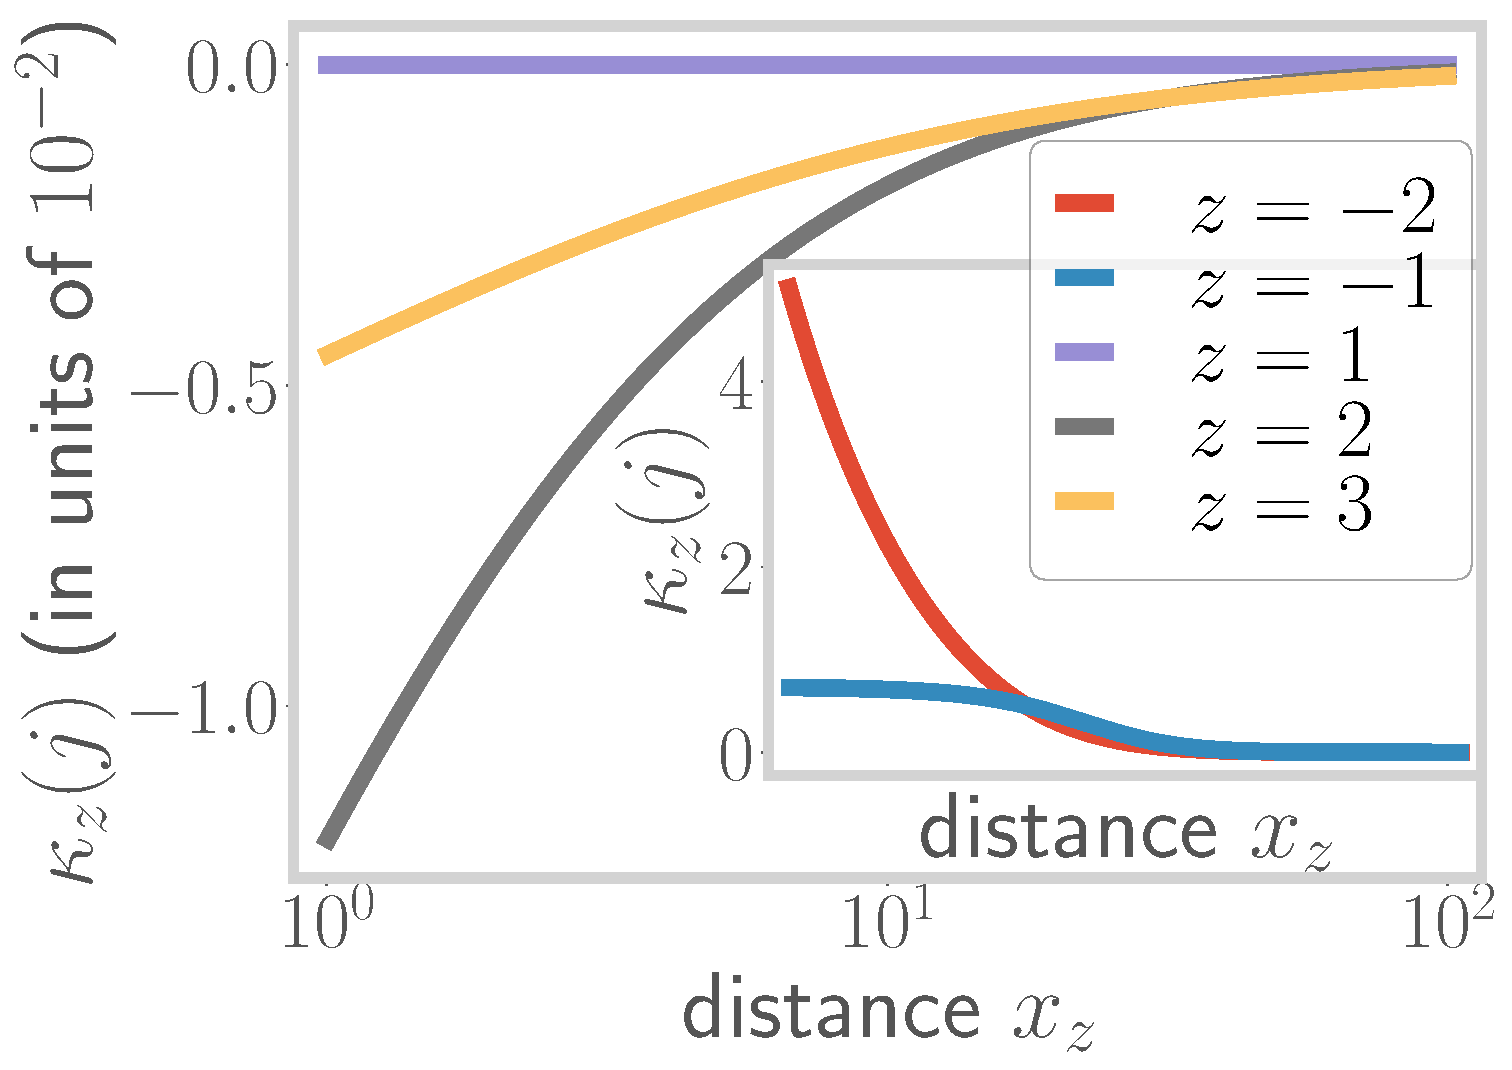
\includegraphics[width=\textwidth]{curvature-pos.pdf}
	\end{minipage}
\end{frame}

\begin{frame}{RG evolution = emergent distance}
	\footcite{maldacena1999large,ryu2006aspects,holzhey_1994}
\begin{itemize}
	\item Distances and curvature can be related to an RG \focus{beta function}\\[10pt]
	\item Amounts to an \focus{explicit demonstration} of the holographic principle\\[10pt]
	\item Sign of curvature is \focus{topological}, can be written in terms of winding numbers\\[10pt]
\end{itemize}
	
\end{frame}

\begin{frame}{Topological nature of geometry-independent term}
	\footcite{luttinger1960ground,luttinger1960fermi,oshikawa2000topological,seki2017topological,anirbanurg1,Heath_2020}
	\[S_{\mathcal{A}_z(j)} = f_z(j) c \alpha L_x - \underbrace{c \log \big|2\sin\left(\pi f_z(j)\phi\right)\big|}_{=Q(\phi),\text{geometry-independent term}}\]
	\begin{itemize}
	\item \(Q(\phi)\) is periodic in the flux \(\phi\), ~ \(\phi=1\) transports a charge across Fermi surface\\[10pt]
	\item pole structure of \(\left(\sin \frac{\pi}{4} - |\sin\left(\pi f_z(j)\right)\phi|\right)^{-1}\) counts number of states \(\longrightarrow\) tracks Luttinger volume\\[10pt]
	\item Luttinger volume is topological, so is \(Q(\phi)\); \(Q(\phi)\) can be expressed in terms of winding numbers
	\end{itemize}
	
\end{frame}

\begin{frame}{}
\section{Future Prospects}
\end{frame}

\begin{frame}{A novel auxiliary model approach}
\begin{itemize}
\only<1>{
	\item Using local impurity models to create bulk lattice models (Bloch's theorem)
		\[ H_\text{bulk} = \sum_i H_\text{local}(i), ~ ~\Psi_\text{bulk}(\vec k) \sim \sum_i e^{i \vec{k}\cdot\vec{r}_i}\Psi_\text{local}(i)\]
	\item Relates bulk correlation functions to those of the auxiliary model\\[20pt]
	\item phase transition in the extended AIM \(\longrightarrow\) phase transition inthe bulk model, \focus{metal-insulator transition} in Hubbard-Heisenberg model\\[20pt]
}
\only<2>{
	\item Should be useful for studying other models of strong-correlations
		\begin{itemize}
			\item periodic Anderson/Kondo models
			\item Heisenberg models\\[20pt]
		\end{itemize}
	\item Another potential application: topologically active systems:
		\begin{itemize}
			\item Fractional quantum hall systems
		\end{itemize}
}
\only<3>{
	\item Method can be made more powerful by using multiple impurities\\[20pt]
	\item Allows entangled liquid-like insulating phases\\[20pt]
	\item Might also provide \(k-\)space resolution 
		\begin{itemize}
			\item partial gapping of Fermi surface?
			\item pseudogap phases\\[20pt]
		\end{itemize}
	\item Extend the formalism towards higher order Greens functions
		\begin{itemize}
			\item two-particle Greens functions, doublon-holon correlations
			\item can provide more info on the MIT
		\end{itemize}
}
\end{itemize}
\end{frame}

\begin{frame}{Heavy-fermion materials}
\begin{itemize}
	\item Materials with very high quasiparticle masses\\[20pt]
	\item Outstanding questions exist about the nature of phases and phase transitions
		\begin{itemize}
			\item microscopic justification of certain phases
			\item theory for the strange metal excitations
			\item microscopic justification for the origin of unconventional superconductivity\\[20pt]
		\end{itemize}
	\item the URG, MERG and auxiliary model methods should prove useful
\end{itemize}
\end{frame}

\begin{frame}{Acknowledgements}
\flushleft
Grateful to\\[10pt]
\begin{itemize}
	\item my collaborators Siddhartha Patra, Anirban Mukherjee, Prof. Arghya Taraphdar, Prof. N. S. Vidhyadhiraja, and \\[10pt]
	\item IISER Kolkata for funding \\[10pt]
\end{itemize}

Special thanks to Prof. Horacio Casini, Prof. Narayan Banerjee and Shibendu G. Chowdhury for some very fruitful discussions.
	
	

	
\end{frame}
	
\begin{frame}[allowframebreaks]{References}
\printbibliography
\end{frame}
\end{document}
